\documentclass[assd_tp3_main.tex]{subfiles}
\geometry{verbose,tmargin=2.25cm,bmargin=2cm,lmargin=2.25cm,rmargin=2cm}
\begin{document}

\subsection{Implementación}

Para realizar la implementación práctica, se utilizó de base el circuito propuesto en las indicaciones del trabajo práctico, realizando las modificaciones pertinentes para su correcto funcionamiento. El diagrama en bloques del circuito es el siguiente.

\todo[inline]{Poner diagrama en bloques con simbolos}

\subsubsection{Filtros Antialiasing - Recuperador}

\todo[inline]{Aca poner el circuito decir que es el mismo, atenua 40dB en 60K lo puse la f de corte en 6K. Por simplicidad se usaron intergradores compensados}

\subsubsection{Diferenciador}

En la implementación propuesta, el modulador posee entrada diferencial (en lugar de una sola entrada referida a masa). Esto permite cancelar bastante el ruido en modo común, lo cual resulta como una ventaja adicional dado que se trabajará con frecuencias de clock de hasta 1MHz, y éste podría provocar interferencias en la señal muestreada con capacitores switcheados de manera no deseada si no se toman algunas consideraciones en el layout del PCB (que se explicará luego). El circuito diferenciador se implementó con amplificadores operacionales, como se muestra a continuación.

\begin{figure}[!ht]
\begin{centering}
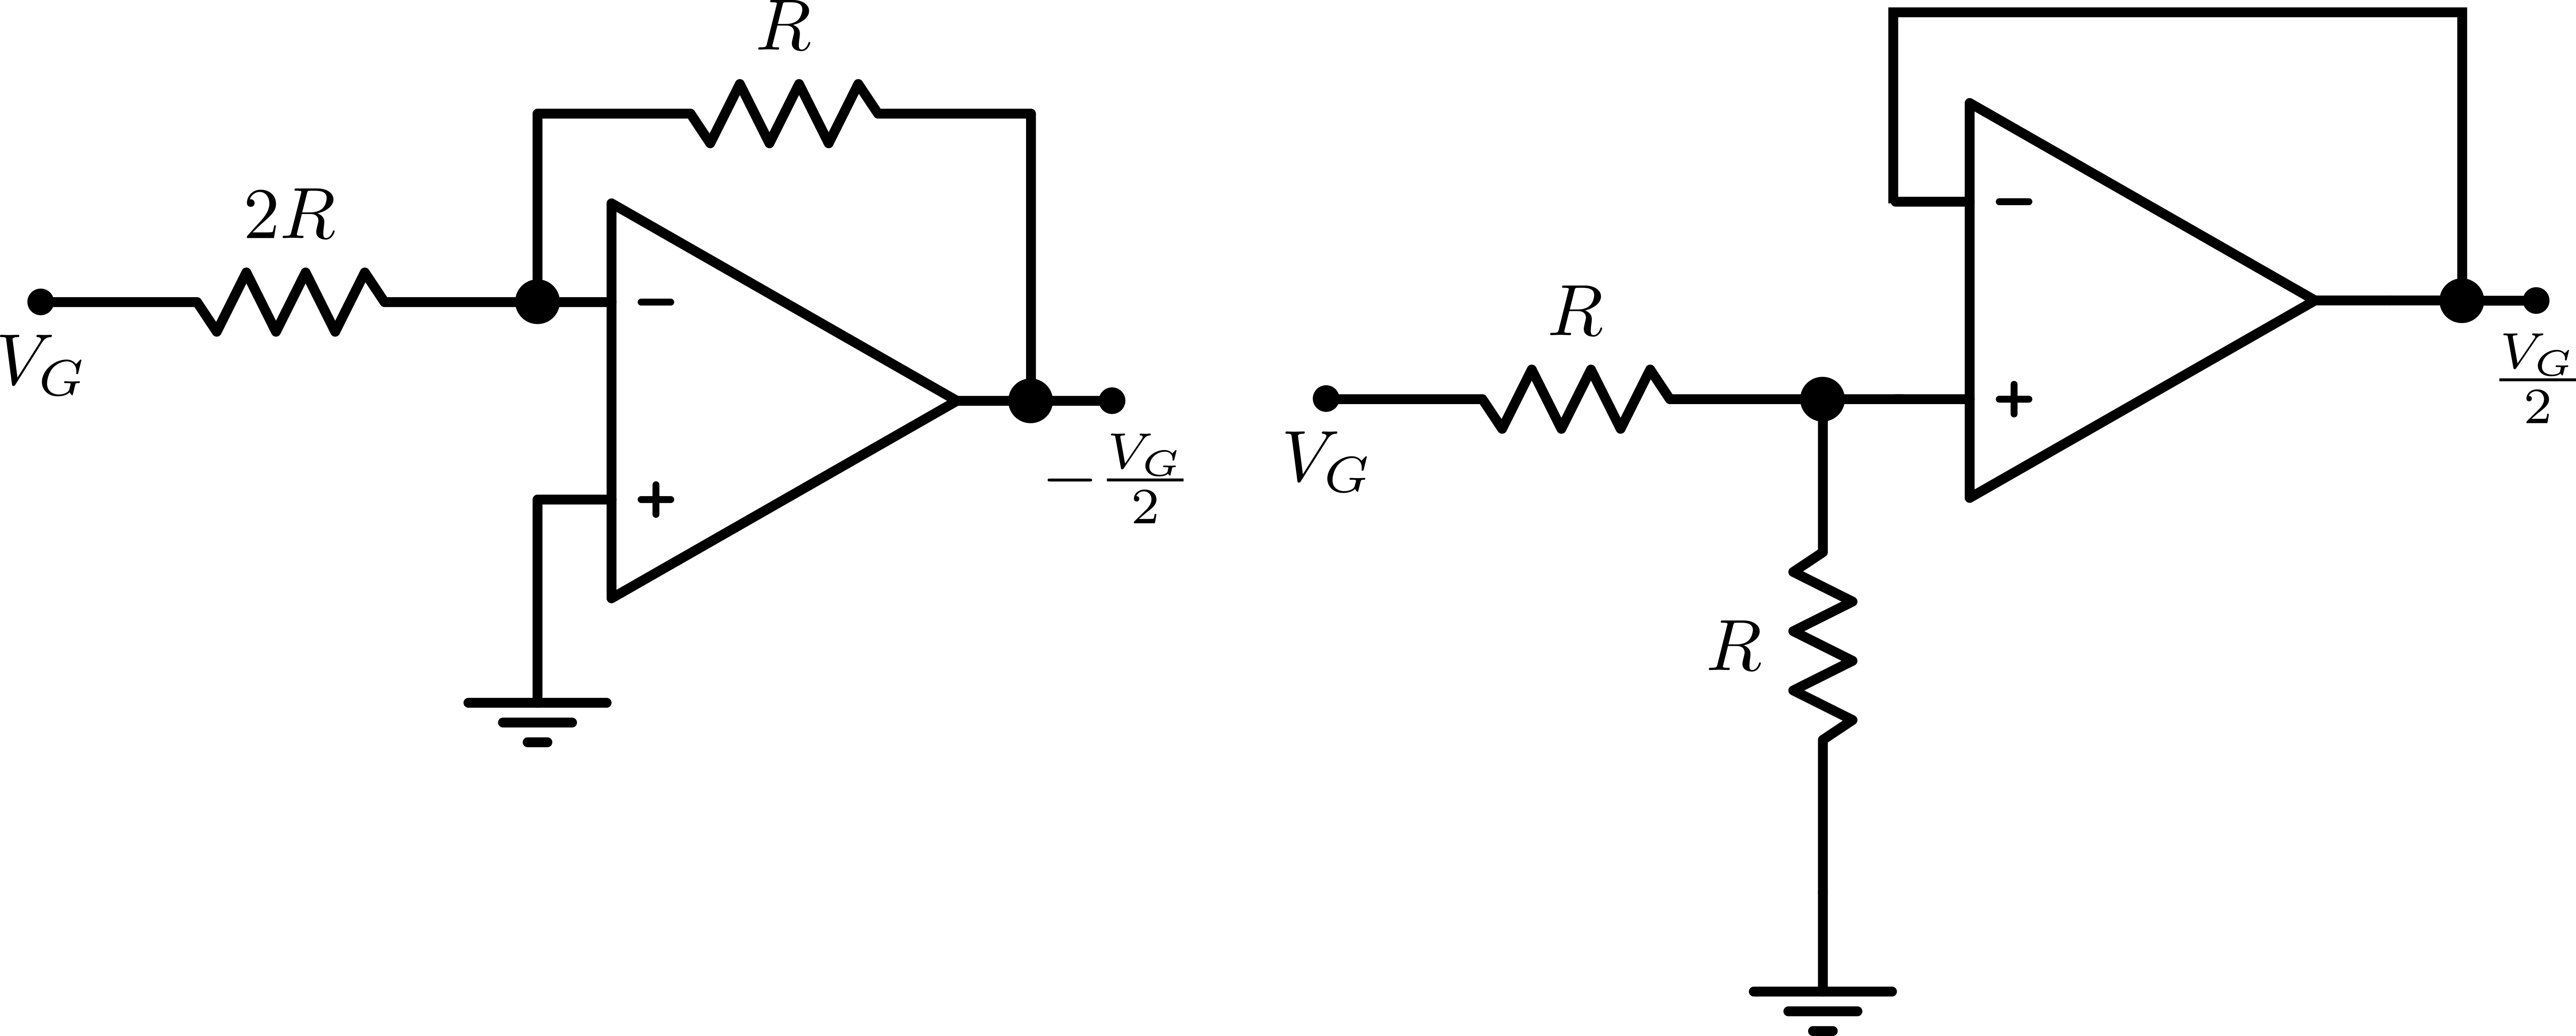
\includegraphics[scale=0.5]{images/ej5/diferenciador.png}
\par\end{centering}
\caption{Generador de señal diferencial}
\end{figure}

\subsubsection{Integrador con switched capacitors (SC)}

La idea se basa en la conmutación de los terminales del capacitor entre tensiones diferentes, que para el análisis deben ser suficientemente estables durante el tiempo T que dura la conmutación. Dicha conmutación suele realizarse con llaves simuladas mediante transistores MOS, pero para simplificar la comprensión se lo esquematiza con llaves ideales, como se muestra a continuación.

\begin{figure}[!ht]
\begin{centering}
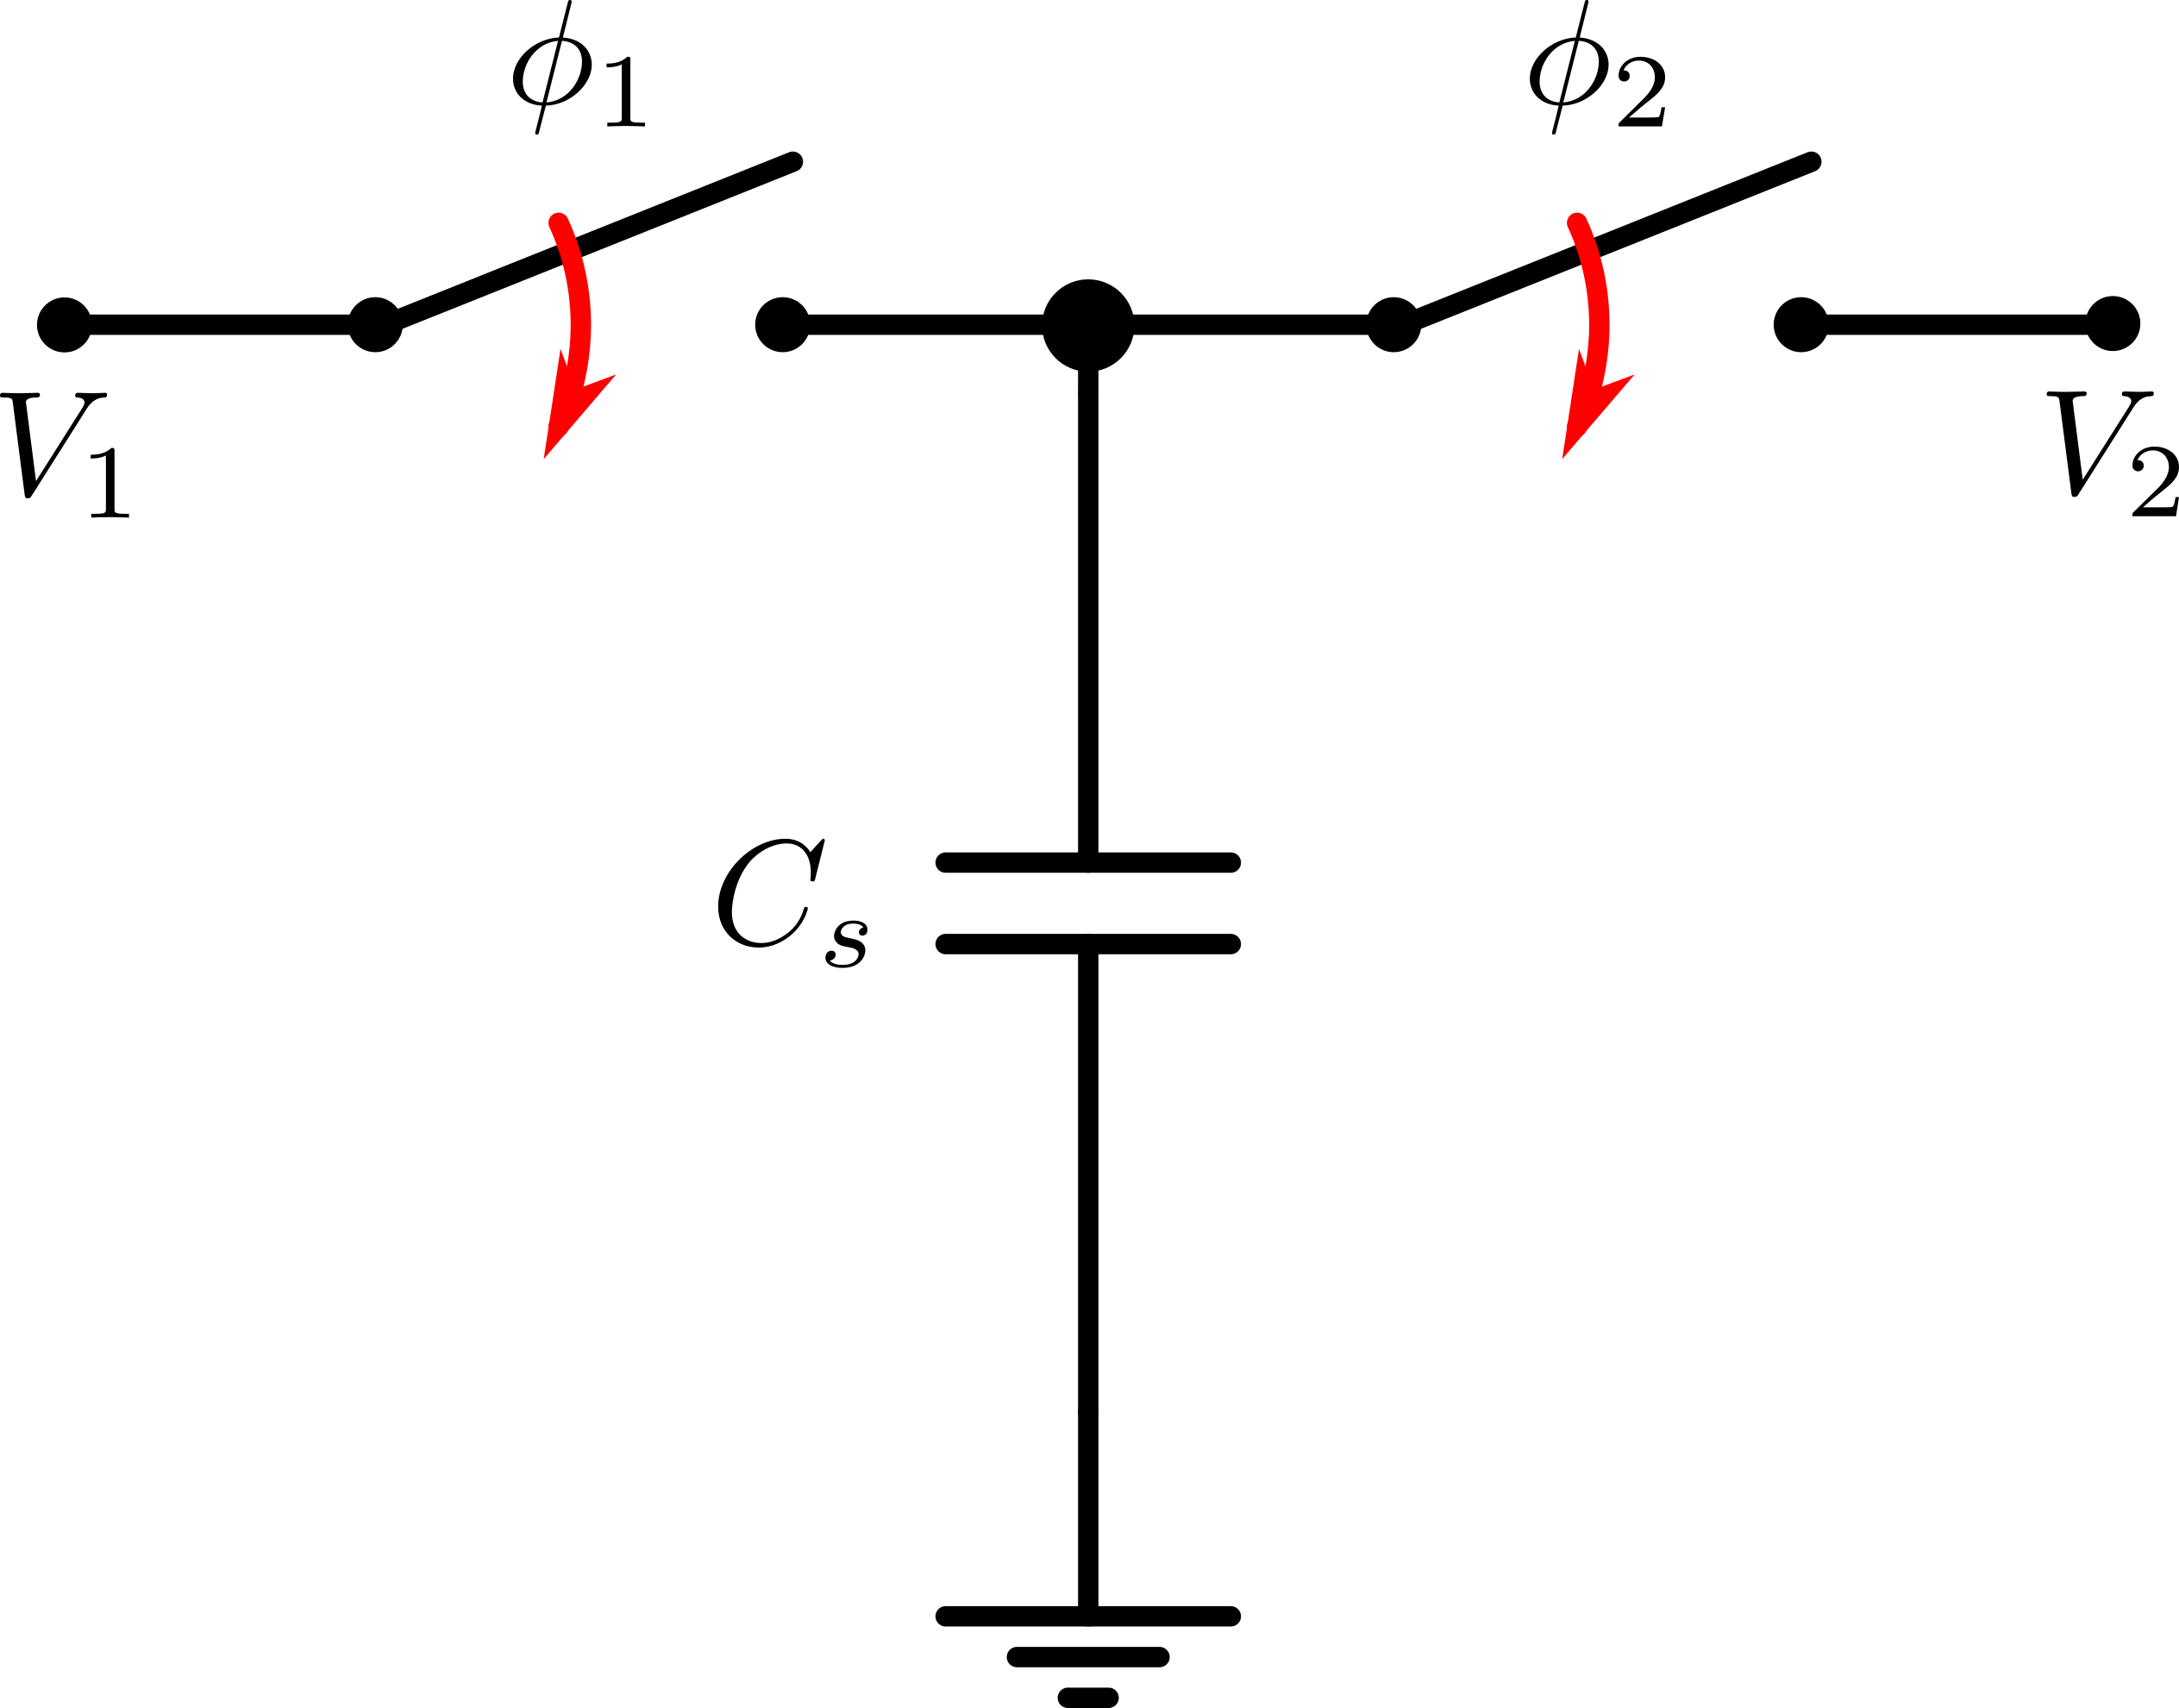
\includegraphics[scale=0.5]{images/ej5/SCBasico.png}
\par\end{centering}
\caption{Esquema de capacitor switcheado}
\end{figure}

Supongase que inicialmente se tiene al capacitor cargado con la tensión $V_2$, con ambos switches abiertos. Luego, se cierrra el switch $\phi_1$, conectando ahora el terminal del capacitor a la tensión $V_1$, durante un tiempo T. La diferencia de carga puede expresarse como:

\[
\Delta Q_1 = C_s \cdot (V_1 - V_2)
\]

Posteriormente se abre $\phi_1$, quedando el capacitor ahora cargado con $V_1$. Ahora se cierra $\phi_2$, conectando el terminal del capacitor a la tensión $V_2$, durante un mismo tiempo T. La diferencia de carga puede expresarse como sigue:

\[
\Delta Q_2 = C_s \cdot (V_1 - V_2)
\]

Observando que $\Delta Q_1 = \Delta Q_2$, la corriente promedio en cada tiempo T debe ser la misma:

\[
i = \frac{\Delta Q_1}{T} = \frac{\Delta Q_2}{T} = \frac{C_s \cdot (V_1 - V_2)}{T}
\]

Despejando según la ley de Ohm, se obtiene la resistencia R equivalente (ya que como se dijo, la carga que circula es la misma):

\[
\frac{V_1 - V_2}{i} = R = \frac{T}{C_s}
\]

Llamaremos T al tiempo de muestreo de las tensiones $V_1$ y $V_2$. Se deja por un lado esta equivalencia, pasando ahora al circuito donde se busca aplicar este sistema.\par 
Para que el circuito se adapte al modelo discreto analizado previamente, se parte del integrador conocido implementado con RC. Se muestra el circuito conocido (ideal) para señales referidas a masa:

\begin{figure}[!ht]
\begin{centering}
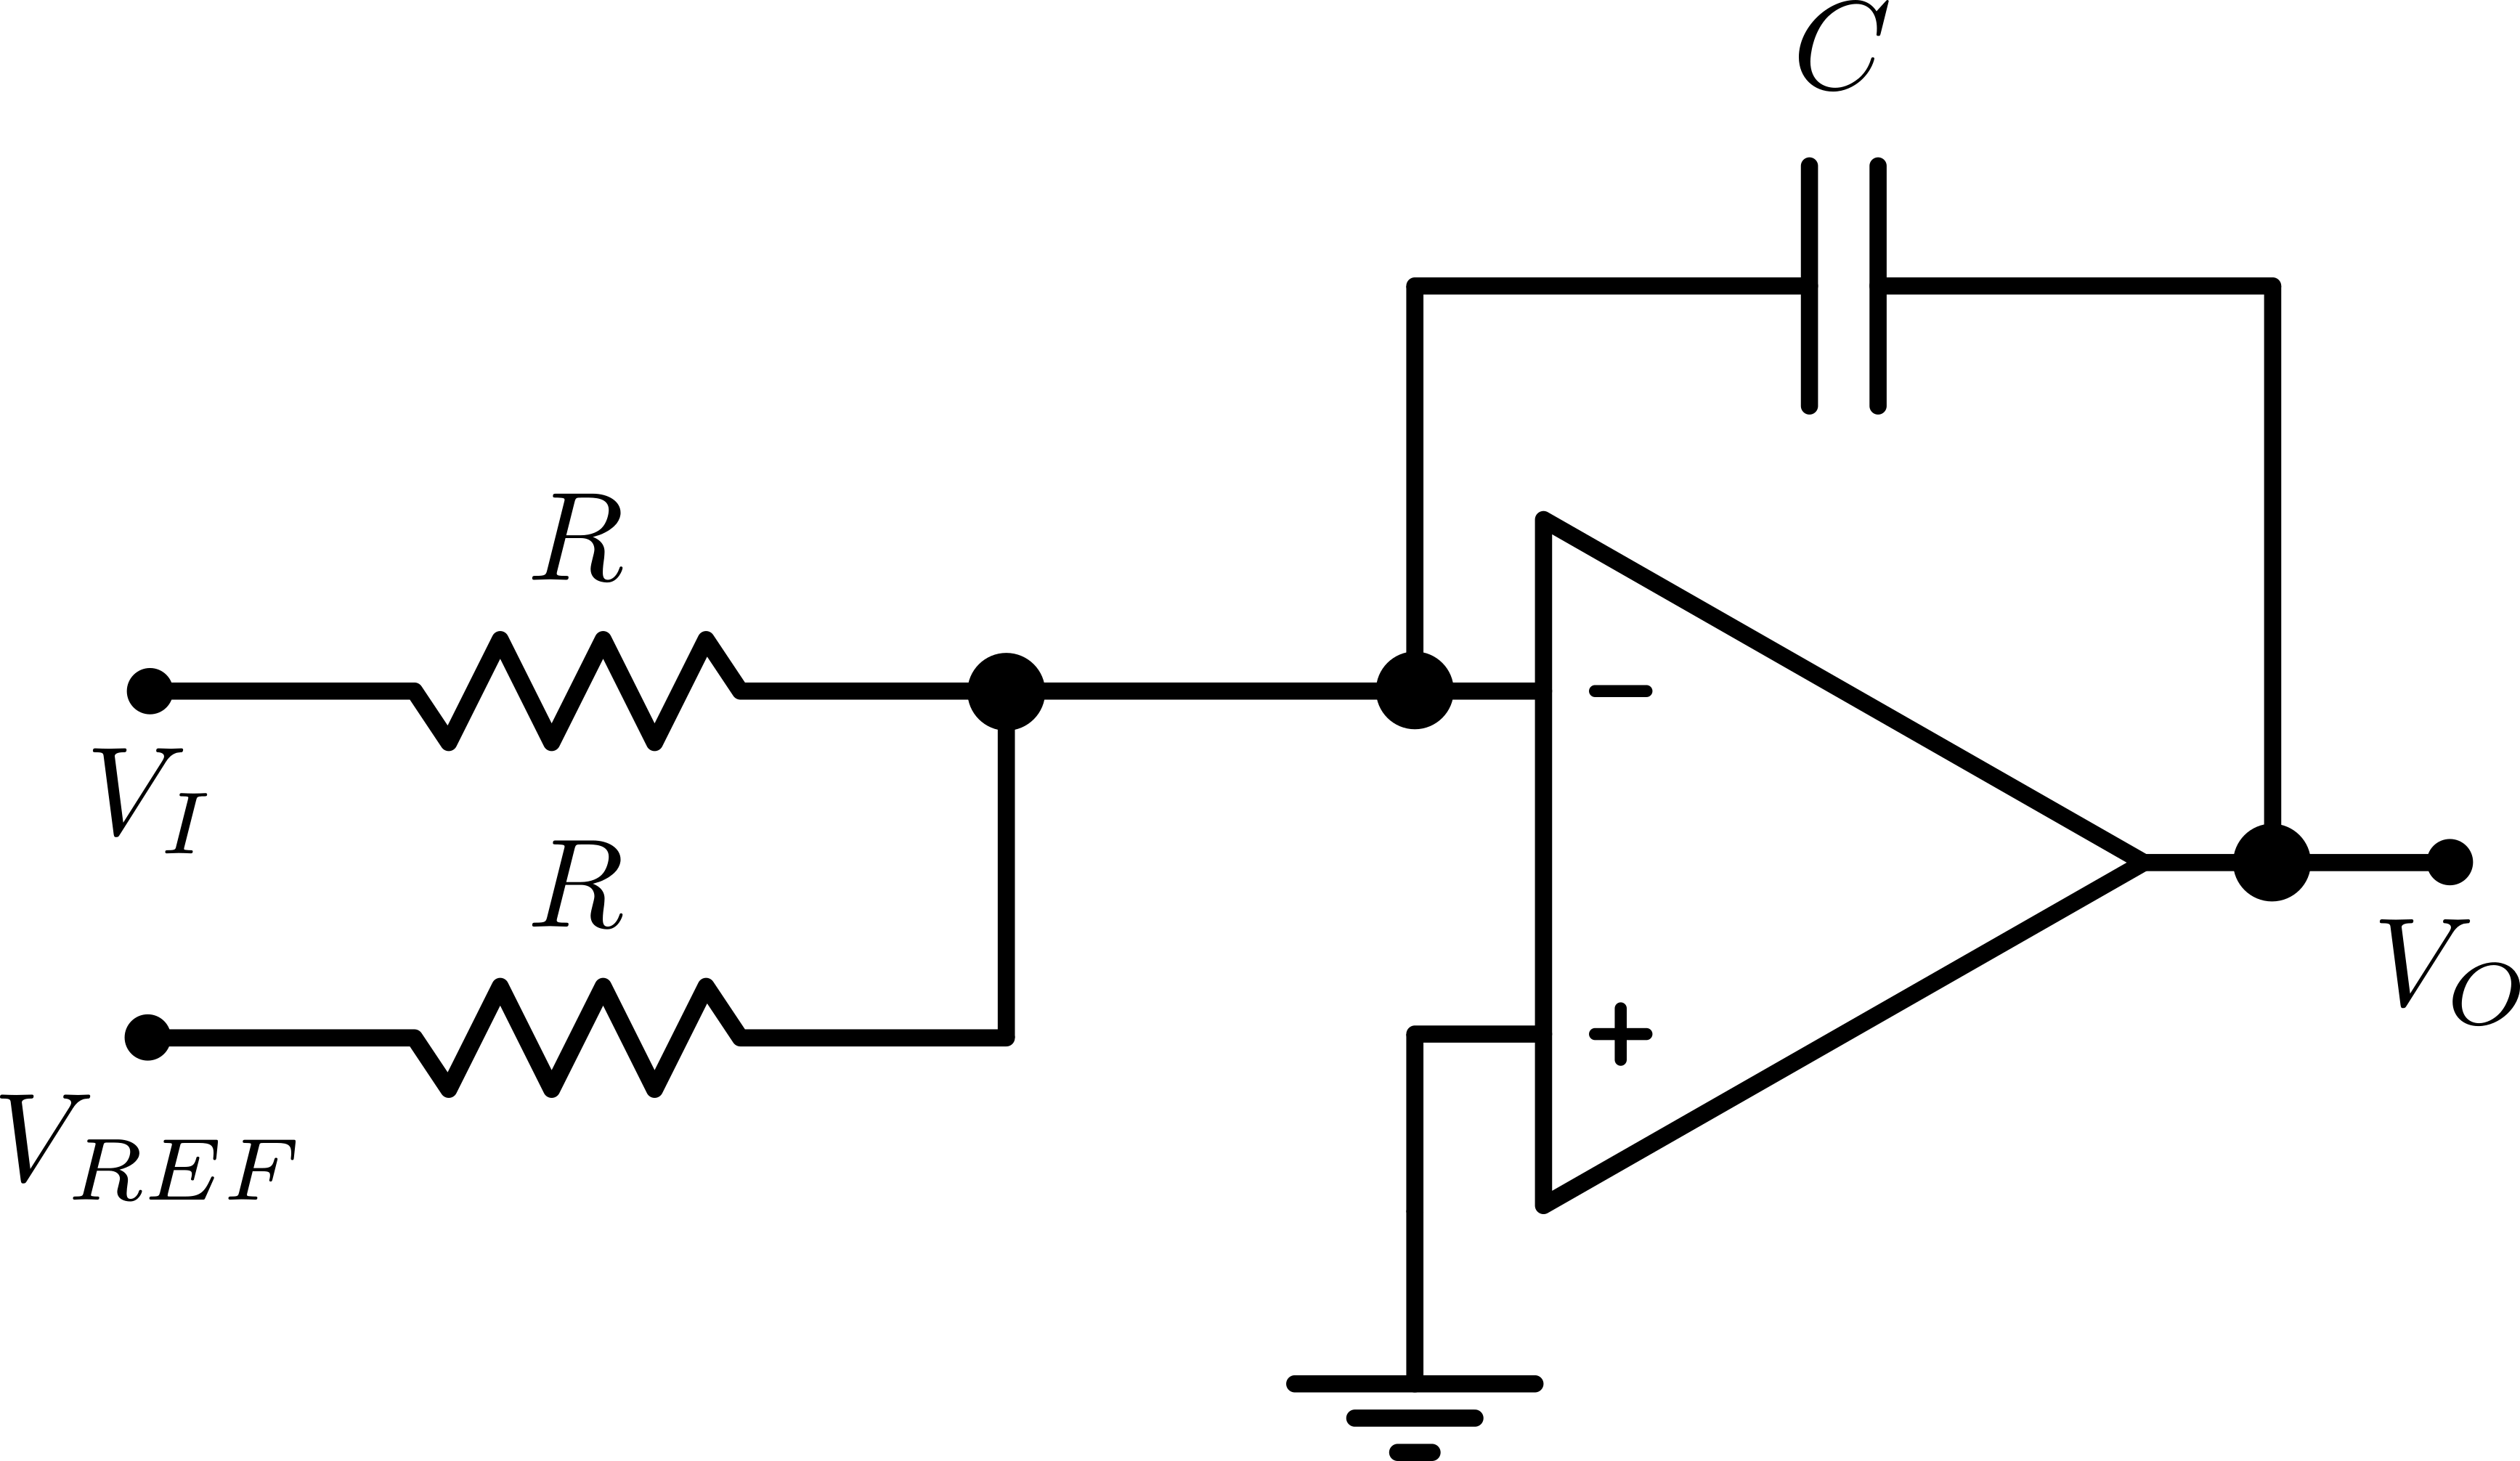
\includegraphics[scale=0.5]{images/ej5/IntegradorBasico.png}
\par\end{centering}
\caption{Circuito integrdor analógico}
\end{figure}


Aplicando la ganancia de tensión conocida para un circuito inversor con operacionales se tiene:

\[
V_O = (V_I+V_{REF}) \cdot \frac{-\frac{1}{sC}}{R} = (V_I + V_{REF}) \cdot -\frac{1}{sCR}
\]

En el caso propuesto, el circuito a implementar es diferencial, como se muestra a continuación.

\begin{figure}[!ht]
\begin{centering}
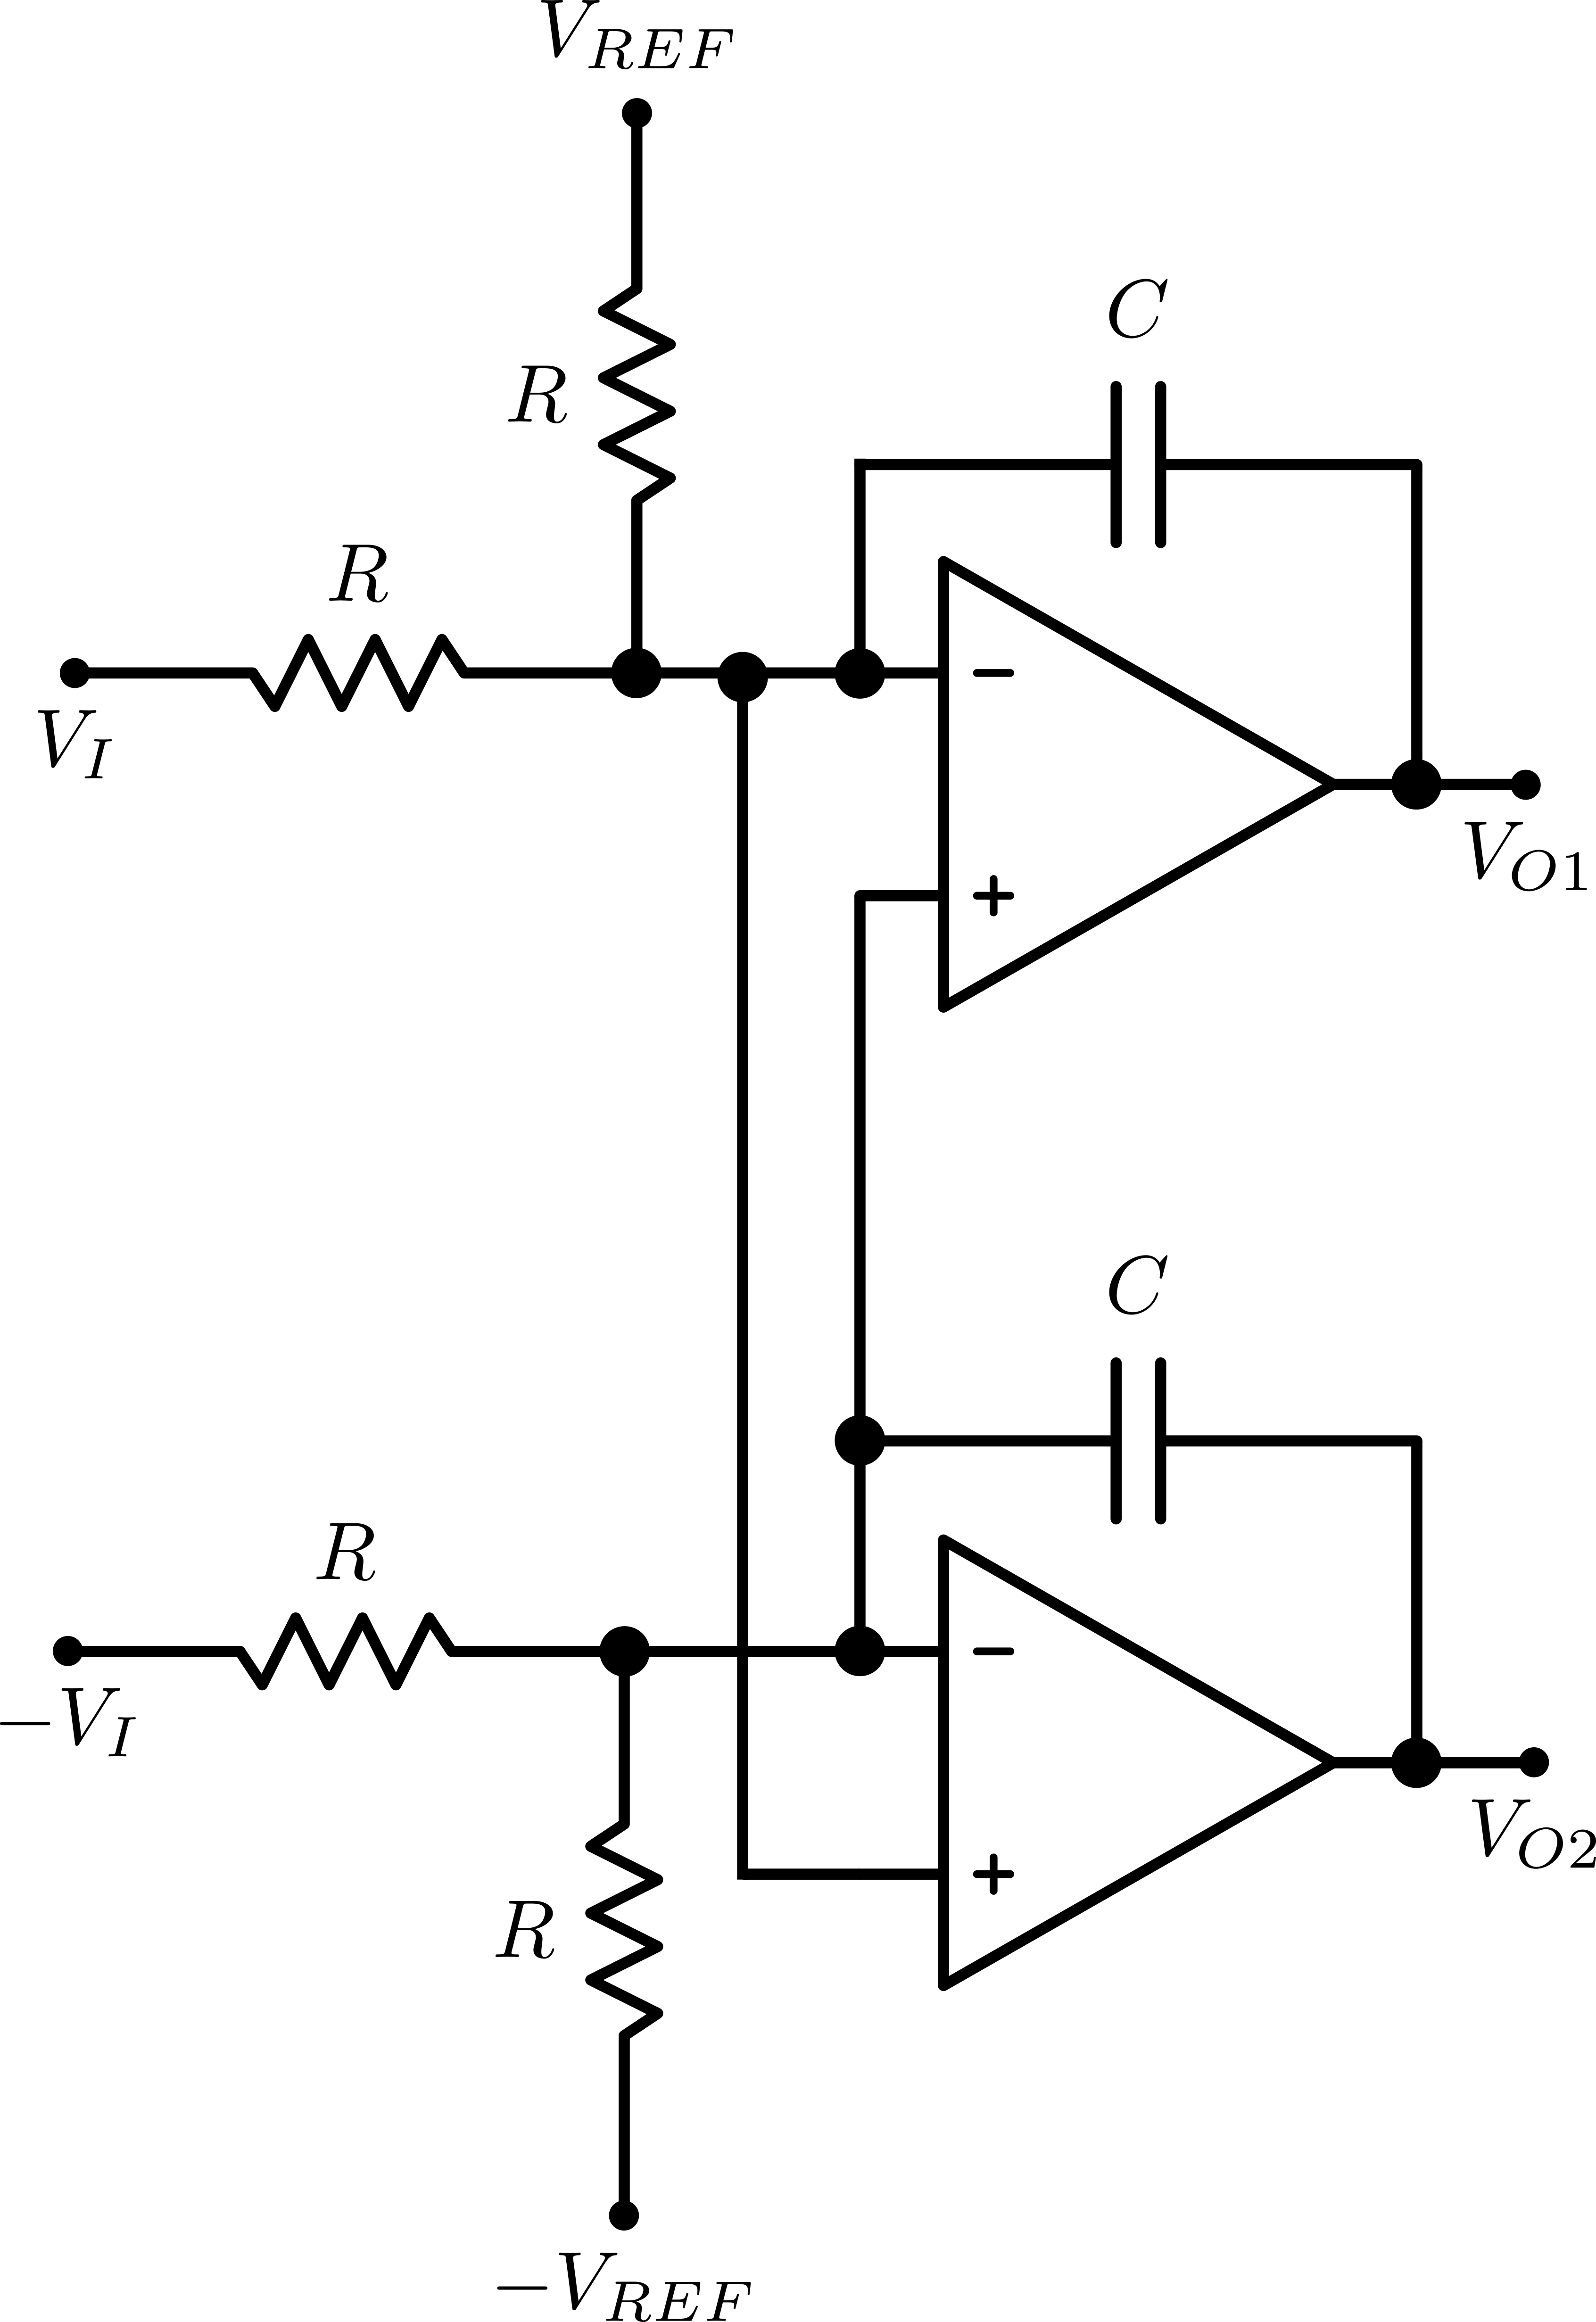
\includegraphics[scale=0.45]{images/ej5/IntegradorDif.png}
\par\end{centering}
\caption{Circuito integrdor diferencial}
\end{figure}

Como se mostró al inicio en el diagrama en bloques, se toma para una realimentación la salida $Q$ (pasada por el DAC) para un lazo y $\overline{Q}$ (también pasada por otro DAC idéntico) para el otro lazo (ya que al ser diferencial, ambos lazos deben ser complementarios). En este caso la salida a considerar $V_{O1} - V_{O2}$ no se observa en forma directa como en el circuito anterior. Pasivando por un lado las tensiones $V_{REF}$, se tiene planteando nodos:

\[
\left\lbrace
\begin{array}{l}
\dfrac{V_I-V_A}{R} + \dfrac{-V_A}{R} = (V_A-V_{O1}) \cdot sC \\
\\
\dfrac{-V_I-V_A}{R} + \dfrac{-V_A}{R} = (V_A-V_{O2}) \cdot sC
\end{array}
\right.
\] 

Restando ambas ecuaciones resulta:

\[
\frac{V_I}{sCR} = \frac{V_{O2}-V_{O1}}{2}
\]

Análogamente, pasivando las tensiones $V_{REF}$:

\[
\frac{V_{REF}}{sCR} = \frac{V_{O2}-V_{O1}}{2}
\]

Luego, por superposición, sumando ambos resultados se tiene finalmente:

\[
V_{O1} - V_{O2} = -\frac{1}{sCR} \cdot (V_I + V_{REF})
\]

Aplicando la transformación bilineal (que es la aproximación discreta de un integrador analógico):

\[
s \simeq \frac{2}{T} \cdot \frac{z-1}{z+1}
\]

Siendo T el período de muestreo. Resulta en la ecuación anterior:

\[
V_{O1}-V_{O2} = -\frac{V_I+V_{REF}}{CR} \cdot \frac{T}{2} \cdot \frac{z+1}{z-1}
\]

Recordando ahora la equivalencia resistiva simulada del capacitor switcheado explicada al inicio (considerando ahora que son 4 switches y no 2, el período es la mitad):

\[
R = \frac{T}{2C_s}
\]

Si se reemplaza en la expresión anterior queda la aproximación al integrador analógico buscada:

\[
V_{O1}-V_{O2} = -\frac{V_I+V_{REF}}{C \cdot \dfrac{T}{2C_s}} \cdot \frac{T}{2} \cdot \frac{z+1}{z-1} = -(V_I + V_{REF}) \cdot \frac{C_s}{C} \cdot \frac{z+1}{z-1}
\]

El circuito que resulta de reemplazar la resistencia por el capacitor $C_s$ es:

\todo[inline]{Poner el circuito diferencial con Cs}

Las llaves $\phi$ se implementaron mediante multiplexores, utilizando la señal de clock como señal de control para la selección de las llaves. El multiplexor que se encontraba disponible es el CD4053.

\subsubsection{Cuantizador de 1 bit}

Se toma la salida del integrador diferencial, y mediante un comparador a lazo abierto se implementa el cuantizador de 1 bit. El circuito implementado es utilizando el comparador LM311, y luego, dicha salida se conecta a un flip-flop D, el cual actúa como latch. El flip-flop D utilizado es el integrado CD4013, alimentado entre +5V y 0V. La alimentación adicional se obtuvo a partir de la entrada de +15V del circuito pasándola por el regulador LM7805.

\todo[inline]{Poner circuito con LM311 y pull up y el flip flop D}

Como se mostrará en las mediciones obtenidas, la salida que se obtiene en este punto del circuito es una señal cuadrada de ancho de pulso modulado (PWM). En los tramos donde la pendiente de la señal es pequeña, las variaciones en la salida del integrador serán menores, por lo que en consecuencia el ancho de los pulsos resultantes es mayor. En los tramos donde la pendiente de la señal es mayor, las variaciones a la salida del integrador son más frecuentes, por lo que el ancho de los pulsos es menor.

\subsubsection{DAC para realimentación}

Las salidas binarias del flip-flop D corresponden a 0V (0 lógico), y +5V (1 lógico). Esta salida (tanto $Q$ y $\overline{Q}$) son convertidas mediante un DAC a -5V (0 lógico) y +5V (1 lógico), siguiendo el esquema propuesto por la bibliografía. Cada DAC es implementado mediante un multiplexor, utilizando las salidas del flip-flop como señales de control.

\todo[inline]{Circuito del DAC}

Se toma la salida de uno de los DAC como señal digital, para luego procesarla por el filtro recuperador (idéntico al antialiasing), para volver a obtener la señal original al quedarnos sólo con el espectro en banda base.

\end{document}